\documentclass[conference]{IEEEtran}

\usepackage[T1]{fontenc}
\usepackage[utf8]{inputenc}
\usepackage{graphicx}
\usepackage{cite}
\usepackage{amsmath,amssymb}
\usepackage{booktabs}
\usepackage{tabularx}
\usepackage{array}
\usepackage{enumitem}
\usepackage{float}
\usepackage{hyperref}
\usepackage{xcolor}
\usepackage{url}

\graphicspath{{./}}

\emergencystretch=2em

\hypersetup{
  colorlinks=true,
  linkcolor=black,
  citecolor=black,
  urlcolor=blue
}

\newcolumntype{P}[1]{>{\raggedright\arraybackslash}p{#1}}

% ── Title ─────────────────────────────────────────────────────────────────────
\title{Intent-to-API Orchestration for Future Telco Networks:\\
A CAPIF-Aware, AI-Native Platform with Empirical\\
Reliability Evaluation}

\author{
\IEEEauthorblockN{T\"{u}rkan Do\u{g}a Durak}
\IEEEauthorblockA{
Centre Tecnol\`{o}gic de Telecomunicacions de Catalunya (CTTC)\\
Castelldefels, Spain\\
\texttt{turkandoga.durak@cttc.es}
}
\and
\IEEEauthorblockN{Engin Zeydan}
\IEEEauthorblockA{
Centre Tecnol\`{o}gic de Telecomunicacions de Catalunya (CTTC)\\
Castelldefels, Spain\\
\texttt{ezeydan@cttc.es}
}
}

\begin{document}
\maketitle

% ── Abstract ──────────────────────────────────────────────────────────────────
\begin{abstract}
Future Internet architectures demand programmable network exposure frameworks
that bridge high-level operator intents to concrete telecom API invocations
without manual payload composition.
This paper presents a cloud-native, CAPIF-aware telco orchestration platform
combining 3GPP CAPIF governance, CAMARA-aligned service semantics, and
LLM-assisted planning under a three-layer deterministic validator.
Evaluation on a 300-entry bilingual ground-truth dataset using six
reliability metrics yields IWSR\,=\,95.7\,\% (GPT-4o-mini),
SCR\,$\geq$\,98.3\,\% and SVR\,$\geq$\,97.0\,\% across all LLM providers,
and SS\,=\,0.973; LLM-assisted mode outperforms the rule-based
deterministic baseline (IWSR\,=\,83.3\,\%) on the diverse 300-entry
evaluation, demonstrating superior robustness to intent phrasing variation.
A multi-provider comparison confirms the schema-grounding mechanism is
substantially provider-agnostic, while the Feedback Engine handles only
payload-level errors — residual failures are Phase\,1 service-routing
errors on ambiguous intents.
Platform and dataset are released as open-source artifacts.
\end{abstract}

\begin{IEEEkeywords}
intent-based networking, CAPIF, CAMARA, NEF, 5G/B5G service exposure,
LLM-assisted orchestration, reliability evaluation, zero-touch automation
\end{IEEEkeywords}

% =============================================================================
\section{Introduction}
% =============================================================================

Beyond-5G and 6G architectures elevate programmable service exposure to a
foundational principle of the Future Internet.
3GPP CAPIF (TS\,23.222)~\cite{3gpp_capif} and the CAMARA
project~\cite{camara2022} define the governance and semantic layers enabling
vertical industries to consume network capabilities through standardised APIs.
Orchestration logic must translate natural-language intents into precisely
structured, multi-field API payloads satisfying strict telecom domain
constraints: E.164 phone formats, enumerated QoS profiles, duration bounds,
and live CAPIF registry membership.

LLMs offer a compelling approach~\cite{maatouk2025,flowmind2023,yao2023,qin2024};
however, probabilistic generation cannot guarantee correctness without
external enforcement~\cite{liu2024,telagentbench2025}.
This paper addresses the gap between LLM planning capability and
telecom-grade reliability.
Our main contributions are: (1)~a working, open-source CAPIF-aware telco
orchestration platform against live CAMARA providers; (2)~a two-phase
schema-grounded LLM planner with a pluggable multi-provider dispatcher;
(3)~a three-layer deterministic validator with a bounded feedback
correction loop; and (4)~six formally defined reliability metrics
constituting a reusable evaluation framework.

% =============================================================================
\section{Related Work}
\label{sec:related}
% =============================================================================

Intent-based networking has been explored at the NFV orchestration level
by Rafiq et al.~\cite{rafiq2020} and Coronado et al.~\cite{coronado2022},
both assuming structured inputs rather than natural language.
OpenCAPIF~\cite{molina2022} and NEFSim~\cite{nefsim2022} provide open
5G exposure infrastructure based on 3GPP NEF~\cite{3gpp_nef}; Turkovic et al.~\cite{turkovic2025} demonstrated
live CAMARA QoD integration with end-to-end latency of 230--340\,ms.
On the LLM side, Maatouk et al.~\cite{maatouk2025} identified hallucination
as a primary risk, Liu et al.~\cite{liu2024} showed GPT-4 achieves only
0.40 compliance on JSON schema tasks without grounding, and
Lee et al.~\cite{telagentbench2025} confirmed multi-turn degradation in
telecom agent scenarios.
No prior work combines live CAPIF integration, LLM planning, deterministic
validation, and a standardised multi-metric reliability framework.

% =============================================================================
\section{Platform Architecture}
\label{sec:arch}
% =============================================================================

\subsection{System Overview}

The platform comprises nine components in four logical tiers
(Fig.~\ref{fig:arch}): an \emph{interface tier} (operator dashboard,
FastAPI backend at port\,8000); a \emph{control-plane tier} (Intent Engine,
LLM Planner, three-layer Validator, Feedback Engine, CAPIF Client);
a \emph{provider tier} (QoD, Location Retrieval, QoS Provisioning,
QoS Profiles via CAMARA); and a \emph{persistence tier} (MongoDB).

\begin{figure}[t]
  \centering
  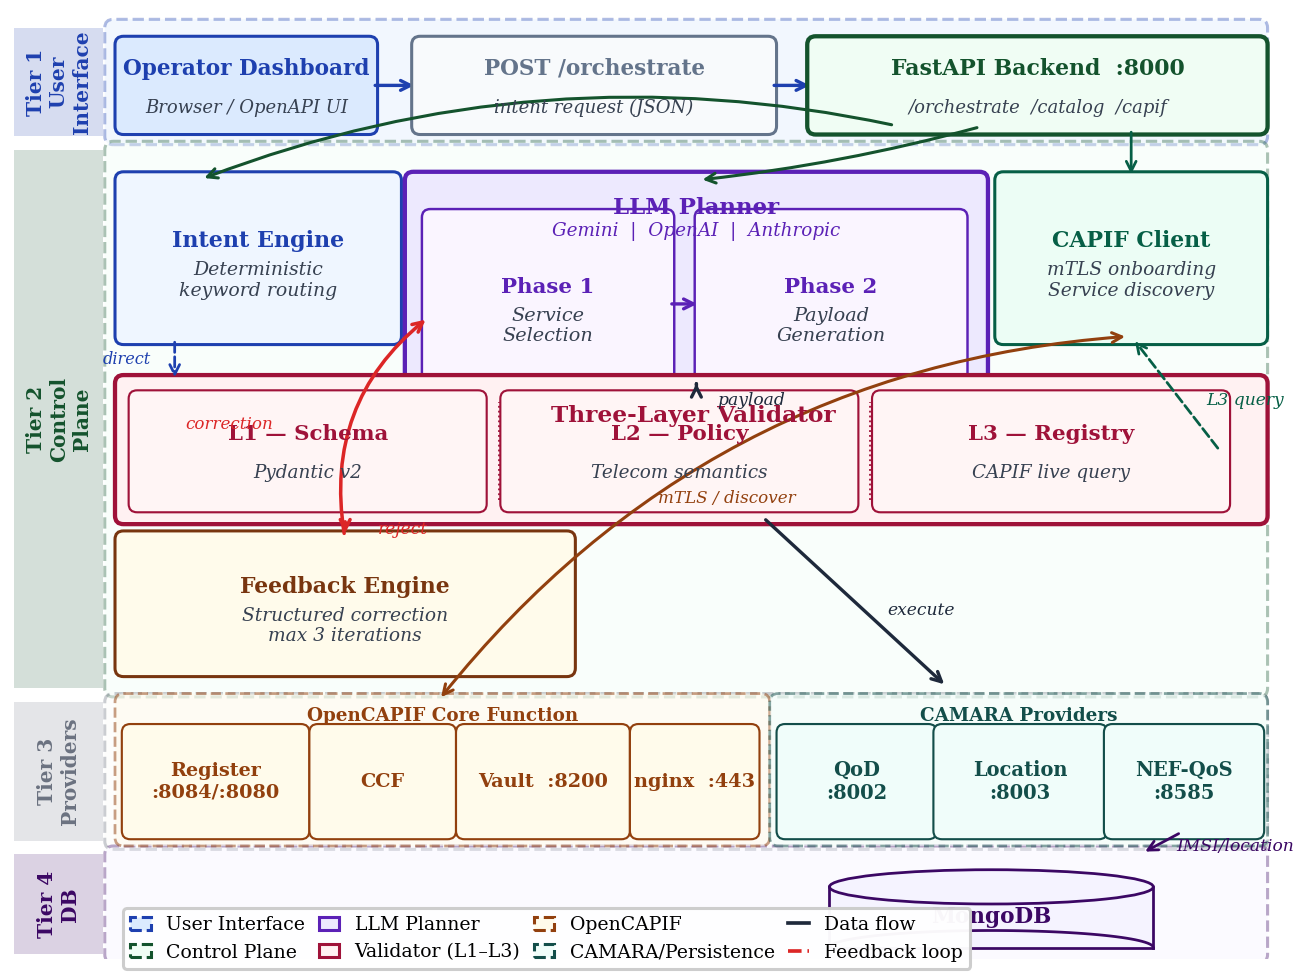
\includegraphics[width=\columnwidth]{nof_fig1_arch.png}
  \caption{System architecture. The CAPIF client follows CAPIF-2e for
  invoker onboarding; CAMARA providers publish through CAPIF-4.
  The three-layer validator (L1--L3) intercepts all LLM-generated
  payloads before any provider call.}
  \label{fig:arch}
\end{figure}

\subsection{CAPIF Integration and CAMARA Services}

The backend acts as a CAPIF Invoker following CAPIF-2e: authenticating,
generating RSA keys and CSR, obtaining an \texttt{apiInvokerId} and
certificate chain, then using mTLS for all discovery and execution.
CAMARA providers publish through CAPIF-4, enabling the L3 validator to
detect hallucinated service identifiers via live registry queries.
Four CAMARA-standardised targets are supported: QoD (v1.1.0), QoS Profiles,
QoS Provisioning (3GPP TS\,29.122), and Location Retrieval (v0.5).

% =============================================================================
\section{LLM-Assisted Orchestration}
\label{sec:llm}
% =============================================================================

\subsection{Two-Phase Schema-Grounded Planning}

Phase\,1 routes the natural-language intent to the correct CAMARA service
using a schema-grounded summary of all available APIs and optional live
CAPIF discovery results.
Phase\,2 generates the full API payload for the selected operation,
injecting the complete CAMARA OpenAPI schema as context.
Grounding Phase\,2 in the exact operation schema is the mechanism that
limits schema errors to under 2\,\% (SCR\,$\geq$\,98.3\,\% across all
providers), confirming the FlowMind hypothesis~\cite{flowmind2023} in a
live telecom environment.
Three LLM providers are supported via a unified dispatcher (Gemini, OpenAI,
Anthropic) switchable at runtime without code changes.

\subsection{Three-Layer Validator and Feedback Loop}

All generated payloads pass three sequential validation tiers before
any provider call:
\textbf{L1 (SCR)} enforces Pydantic\,v2 schema, types, and field constraints;
\textbf{L2 (SVR)} applies eight telecom semantic rules (E.164, QoS enum,
duration 1--7200\,s, IPv4 unicast);
\textbf{L3 (HR)} queries the live CAPIF registry for service existence.
On failure, the Feedback Engine constructs a structured correction prompt
with layer-tagged error messages and retries up to three iterations.
This separation between probabilistic LLM reasoning and deterministic
constraint enforcement is the central property enabling quantified
reliability guarantees.

% =============================================================================
\section{Reliability Evaluation}
\label{sec:eval}
% =============================================================================

\subsection{Metrics and Dataset}

Six metrics formalise intent-to-API reliability:
IWSR (end-to-end correctness), SCR (schema compliance), SVR (semantic
validity), HR (hallucination rate), SS (output stability, $k$ repeated
runs), and RRF (feedback recovery).
The evaluation dataset contains 300 manually crafted bilingual entries
across four CAMARA services, three difficulty levels (easy / medium /
hard), and eight E.164 country codes (+1, +30, +33, +34, +44, +49,
+81, +90) — covering Greek, Turkish, Spanish, US, UK, German, Japanese,
and French number formats.
Entries are distributed as: QoD\,=\,100, Location\,=\,75,
QoS\,Profiles\,=\,50, QoS\,Provisioning\,=\,50, Edge\,Cases\,=\,25.

\subsection{Results}

\begin{table}[t]
\centering
\caption{Reliability Metrics: Deterministic vs.\ LLM-Assisted (300 entries)}
\label{tab:results}
\small
\begin{tabular}{lrr}
\toprule
\textbf{Metric} & \textbf{Deterministic} & \textbf{LLM (Claude Haiku\,4.5)} \\
\midrule
IWSR  &  83.3\,\% &  94.7\,\% \\
SCR   & 100.0\,\% &  98.7\,\% \\
SVR   & 100.0\,\% &  98.7\,\% \\
HR    &  16.7\,\%\textsuperscript{a} &   4.0\,\% \\
SS    &     0.962 &     0.925 \\
RRF   &    N/A    &  60.0\,\%\textsuperscript{b} \\
Latency & $<$1\,ms & $\approx$3\,s \\
\bottomrule
\end{tabular}
\vspace{2pt}
\noindent\footnotesize
\textsuperscript{a}Deterministic HR counts intents unresolved by keyword
mapping (no hallucination; L3 rejects unmatched service identifiers).
\textsuperscript{b}Feedback Engine recovered 3 of 5 payload corrections.
Stratified IWSR (Haiku): easy\,=\,100\,\%, medium\,=\,100\,\%,
hard\,=\,87.0\,\%.
\end{table}

On the diverse 300-entry dataset, the LLM-assisted mode
(Claude\,Haiku\,4.5) achieves IWSR\,=\,94.7\,\%, outperforming the
deterministic baseline (IWSR\,=\,83.3\,\%), which degrades on
phrasings outside its keyword vocabulary.
Deterministic mode retains perfect SCR\,=\,SVR\,=\,100\,\% but maps
16.7\,\% of intents to incorrect or unregistered service identifiers
(counted as HR), yielding the lower IWSR.
LLM-assisted mode achieves SCR\,=\,SVR\,=\,98.7\,\%, confirming that
Phase\,2 schema grounding limits payload-level errors to under 2\,\%.
The Feedback Engine recovered 3 of 5 triggered corrections
(RRF\,=\,60\,\%), leaving 2 unrecovered schema failures.
Stratified results reveal that hard-difficulty entries drive most
failures (hard IWSR\,=\,87.0\,\% vs.\ 100\,\% at easy and medium),
consistent with intentionally ambiguous cross-service intents.

\begin{table}[t]
\centering
\caption{Multi-LLM Reliability Comparison (300 entries)}
\label{tab:multilm}
\small
\begin{tabular}{lrrrrr}
\toprule
\textbf{Provider} & \textbf{IWSR} & \textbf{SCR} & \textbf{SVR} &
\textbf{HR} & \textbf{SS} \\
\midrule
Deterministic        &  83.3\,\% & 100.0\,\% & 100.0\,\% & 16.7\,\%\textsuperscript{$\dagger$} & 0.962 \\
GPT-4o-mini          & \textbf{95.7\,\%} &  98.3\,\% &  97.3\,\% & 2.3\,\% & \textbf{0.973} \\
Claude\,Haiku\,4.5  &  94.7\,\% & \textbf{98.7\,\%} & \textbf{98.7\,\%} & 4.0\,\% & 0.925 \\
Gemini\,2.5\,Flash  &  94.7\,\% &  98.7\,\% &  97.0\,\% & 3.0\,\% & 0.943 \\
\bottomrule
\end{tabular}
\vspace{2pt}
\noindent\footnotesize
\textsuperscript{$\dagger$}Deterministic HR reflects unmatched keyword
intents rejected by the L3 CAPIF registry, not LLM hallucination.
\end{table}

Table~\ref{tab:multilm} compares all four modes on the 300-entry dataset.
SCR\,$\geq$\,98.3\,\% and SVR\,$\geq$\,97.0\,\% across all LLM providers
confirm that Phase\,2 schema grounding is substantially provider-agnostic.
Notably, SVR\,$<$\,SCR for GPT-4o-mini (97.3\,\% vs.\ 98.3\,\%) and
Gemini (97.0\,\% vs.\ 98.7\,\%), indicating that the semantic L2
validator catches payload-format violations missed by Pydantic\,v2 alone.
Feedback recovery rates vary by provider (RRF\,=\,28.6--60.0\,\%),
reflecting the degree to which each LLM benefits from structured
layer-tagged correction prompts.
Fig.~\ref{fig:services} breaks IWSR down by CAMARA service for
Claude\,Haiku\,4.5: Location\,Retrieval, QoS\,Profiles, and
QoS\,Provisioning reach 100\,\%, while QoD\,Sessions (88\,\%) and
edge cases (84\,\%) concentrate failures at the Phase\,1 routing boundary,
confirming that payload generation is not the limiting factor.

\begin{figure}[t]
  \centering
  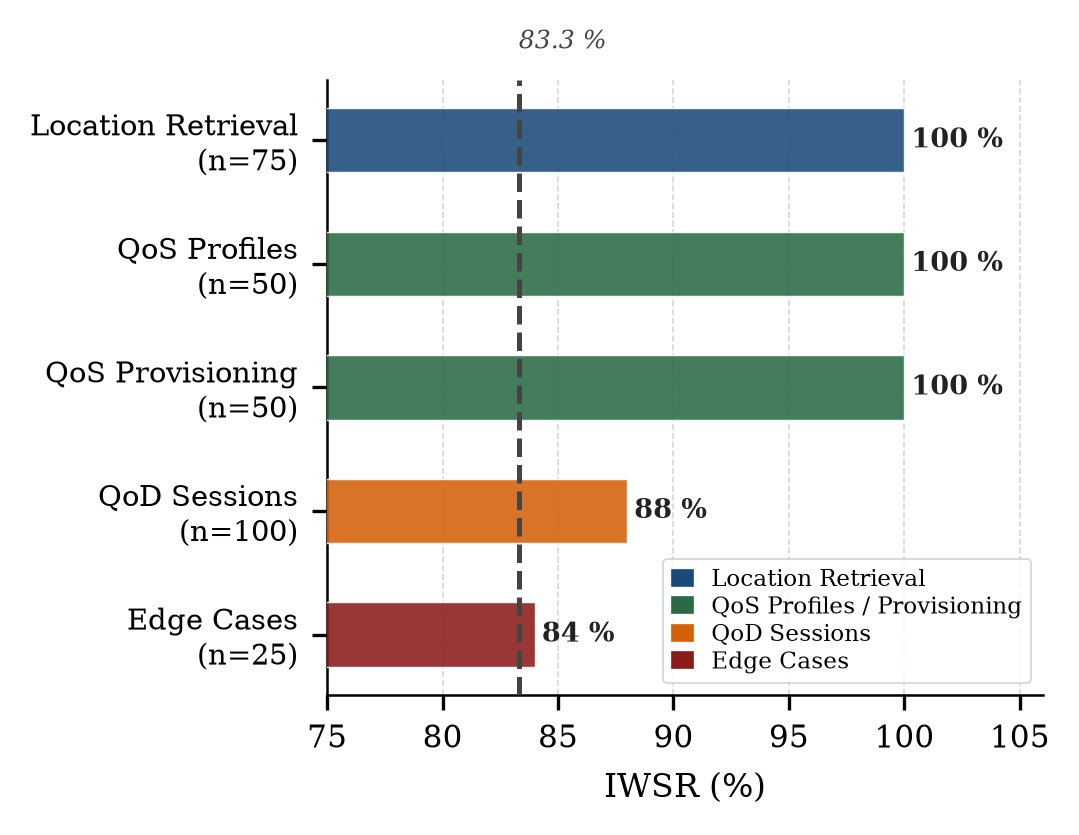
\includegraphics[width=\columnwidth]{nof_fig_services.png}
  \caption{Per-service IWSR breakdown for Claude\,Haiku\,4.5
  ($n$\,=\,300, dashed line\,=\,deterministic baseline 83.3\,\%).
  Location\,Retrieval, QoS\,Profiles, and QoS\,Provisioning each achieve
  100\,\%; QoD\,Sessions (88\,\%) and edge cases (84\,\%) reveal the
  Phase\,1 service-routing boundary as the primary failure locus.}
  \label{fig:services}
\end{figure}

% =============================================================================
\section{Discussion and Conclusion}
\label{sec:conclusion}
% =============================================================================

The central finding is that LLM-assisted orchestration outperforms
the deterministic baseline on the 300-entry diverse dataset
(IWSR\,=\,94.7--95.7\,\% vs.\ 83.3\,\%), reversing the 60-entry result
where deterministic achieved 100\,\% on hand-crafted, templated intents.
This inversion demonstrates the brittleness of keyword-based intent
resolution at scale and motivates the LLM planning approach.
Among LLM providers, GPT-4o-mini leads on IWSR (95.7\,\%) and stability
(SS\,=\,0.973); Claude\,Haiku\,4.5 achieves the highest SVR (98.7\,\%)
and best Feedback Engine recovery rate (RRF\,=\,60\,\%).

Fig.~\ref{fig:difficulty} stratifies IWSR by difficulty level.
All LLM providers exceed the deterministic baseline at every tier;
the advantage widens at hard difficulty (LLM: 87--94\,\% vs.\
deterministic overall: 83.3\,\%), where diverse phrasings exhaust
the keyword matcher most severely.

\begin{figure}[t]
  \centering
  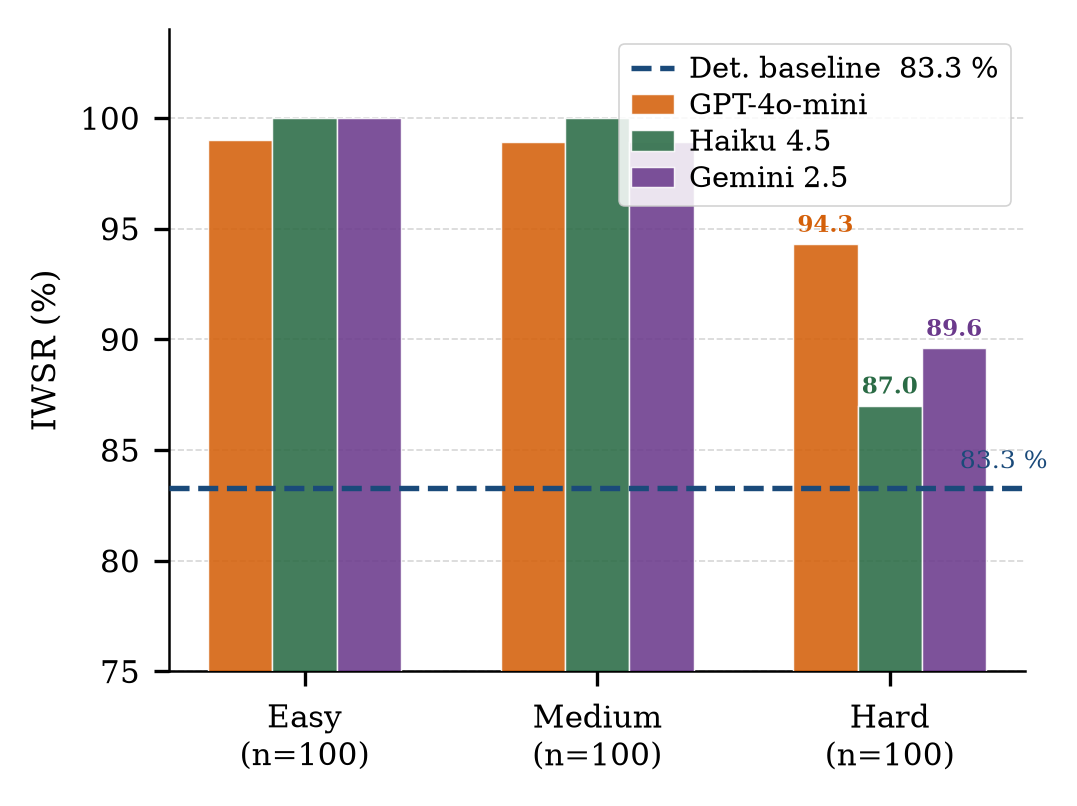
\includegraphics[width=\columnwidth]{nof_fig_difficulty.png}
  \caption{IWSR by difficulty level ($n=100$ per tier, 300 total).
  All LLM providers exceed the deterministic baseline (dashed, 83.3\,\%)
  at every level. The gap widens at hard difficulty, where free-form
  phrasings and the QoD/QoS\,Provisioning routing boundary
  are the primary failure points.}
  \label{fig:difficulty}
\end{figure}

Service-level analysis (Haiku) shows that Location\,Retrieval,
QoS\,Profiles, and QoS\,Provisioning each reach IWSR\,=\,100\,\%, while
QoD\,Sessions (88.0\,\%) and edge cases (84.0\,\%) drive most failures ---
confirming residual errors concentrate at the Phase\,1 routing boundary,
not in payload generation.
Cross-lingual performance is robust: EN\,=\,95.4\,\% and
TR\,=\,93.9\,\% (Haiku), confirming bilingual generalisation without
any translation pre-processing.

This work presents the first empirical reliability evaluation of
LLM-based intent-to-API translation in a live CAPIF-compliant 5G
environment under simultaneous schema, semantic, and registry constraints.
The six-metric framework (IWSR, SCR, SVR, HR, SS, RRF) is reusable
across any intent-to-API orchestration system.
Future work includes integration of open-weight models, 3GPP ZSM
closed-loop control~\cite{etsi_zsm}, and evaluation on real operator
intent logs.

All source code, dataset, and evaluation scripts are available at:
\url{https://github.com/doadurak/mini-telco-platform}.

% =============================================================================
\bibliographystyle{IEEEtran}
\bibliography{references}

\end{document}
